\documentclass[10pt,spanish,aspectratio=1610]{beamer}
\usepackage[utf8]{inputenc}
\usepackage{amsmath}
\usepackage{graphicx}
\usepackage{amssymb}
\usepackage[spanish]{babel}
\spanishdecimal{.}
\usepackage{subfig}
\usepackage{fancyhdr}
\usepackage{pstricks}
\usepackage{color}
\usepackage[ruled]{algorithm2e}
\usepackage{listings}
\usepackage{multicol}
\usepackage{xcolor}

\definecolor{graywhite}{rgb}{0.9529,0.9607,0.9686}
\definecolor{bluegray}{rgb}{0.6823, 0.7411, 0.8}
\definecolor{darkred}{rgb}{0.7372, 0.2392, 0.2392}
\definecolor{bluedark}{rgb}{0.294, 0.4705, 0.6407}
\definecolor{darkgreen}{rgb}{0.1764, 0.5294, 0.0901}
\lstset{
  backgroundcolor=\color{graywhite},   % choose the background color; you must add \usepackage{color} or \usepackage{xcolor}; should come as last argument
  basicstyle=\footnotesize,        % the size of the fonts that are used for the code
  breakatwhitespace=false,         % sets if automatic breaks should only happen at whitespace
  breaklines=true,                 % sets automatic line breaking
  captionpos=b,                    % sets the caption-position to bottom
  commentstyle=\color{darkgreen},    % comment style
  keepspaces=true,                 % keeps spaces in text, useful for keeping indentation of code (possibly needs columns=flexible)
  keywordstyle=\color{darkred},       % keyword style
  language=Octave,                 % the language of the code
  morekeywords={*,...},            % if you want to add more keywords to the set
  numbers=left,                    % where to put the line-numbers; possible values are (none, left, right)
  numbersep=7pt,                   % how far the line-numbers are from the code
  numberstyle=\tiny\color{bluedark}, % the style that is used for the line-numbers
  showspaces=false,                % show spaces everywhere adding particular underscores; it overrides 'showstringspaces'
  showstringspaces=false,          % underline spaces within strings only
  showtabs=false,                  % show tabs within strings adding particular underscores
  stepnumber=1,                    % the step between two line-numbers. If it's 1, each line will be numbered
  stringstyle=\color{bluedark},     % string literal style
  frame=single,
  rulecolor=\color{bluegray},
  tabsize=2,                   % sets default tabsize to 2 spaces
  xleftmargin=1cm,
  xrightmargin=0.5cm,
  framexleftmargin=0.5cm,
  extendedchars=true,
  literate={á}{{\'a}}1 {é}{{\'e}}1 {í}{{\'i}}1 {ó}{{\'o}}1 {ú}{{\'u}}1 {Á}{{\'A}}1 {É}{{\'E}}1 {Í}{{\'I}}1 {Ó}{{\'O}}1 {Ú}{{\'U}}1,
}

\DeclareMathOperator{\atantwo}{atan2}
\setbeamercolor{block title}{fg=white,bg=blue!70!black}
\setbeamercolor{block body}{fg=black, bg=blue!10!white}
\setbeamertemplate{blocks}[rounded][shadow=false]
\setbeamercovered{transparent}
\beamertemplatenavigationsymbolsempty
\setbeamertemplate{frametitle}{
  \leavevmode
  \hbox{\begin{beamercolorbox}[wd=0.6\paperwidth,left]{frametitle}
    \usebeamerfont{frametitle}\insertframetitle
  \end{beamercolorbox}
  \begin{beamercolorbox}[wd=0.4\paperwidth,center]{frametitle}
    \usebeamerfont{frametitle}\small{\thesection . \insertsectionhead}
  \end{beamercolorbox}  } }
\setbeamertemplate{footline}{
  \leavevmode%
  \hbox{%
    \begin{beamercolorbox}[colsep=-0.5pt,wd=.33\paperwidth,ht=3ex,dp=1.5ex,center]{author in head/foot}%
      \usebeamerfont{author in head/foot}\insertshortauthor~~ (\insertshortinstitute)
    \end{beamercolorbox}%
    \begin{beamercolorbox}[colsep=-0.5pt,wd=.34\paperwidth,ht=3ex,dp=1.5ex,center]{date in head/foot}%
      \usebeamerfont{author in head/foot}\insertshorttitle
    \end{beamercolorbox}%
    \begin{beamercolorbox}[colsep=-0.5pt,wd=.33\paperwidth,ht=3ex,dp=1.5ex,right]{author in head/foot}%
      \usebeamerfont{author in head/foot}\insertshortdate{} \hspace*{2em}\scriptsize{\insertframenumber{}}\hspace*{1ex}
    \end{beamercolorbox}
  }
}

\begin{document}
\renewcommand{\tablename}{Tabla}
\renewcommand{\figurename}{Figura}

\title[Etapa 02 - ROS y Takeshi]{ETAPA 02\\La plataforma ROS y el robot Takeshi}
\author[Marco Negrete]{Instructor: Marco Antonio Negrete Villanueva}
\institute[FI, UNAM]{Programa Espacial Universitario, UNAM}
\date[CIRE 2022]{Consurso Iberoamericano de Robótica Espacial 2022\\\url{https://github.com/mnegretev/CIRE2022}}

\begin{frame}
\titlepage
\end{frame}

\begin{frame}
  \Large{Objetivos:}
  \normalsize
  \[\]
  \textbf{Objetivo General:} Que los participantes se familiaricen con las herramientas de software que se usarán durante el concurso. 
  \\
  \textbf{Objetivos Específicos:}
  \begin{itemize}
  \item Revisar la plataforma ROS y el software de control de versiones Git
  \item Dar un panorama general del hardware y software con que cuenta el robot Toyota HSR (Takeshi)
  \item Aprender a interactuar con los sensores y actuadores del robot mediante ROS:
    \begin{itemize}
    \item Base móvil omnidireccional
    \item Sensor Lidar
    \item Cámaras RGB y RGB-D
    \item Manipulador
    \end{itemize}
  \end{itemize}
\end{frame}

\begin{frame}
  \Large{Contenido}
  \normalsize
  \[\]

  \tableofcontents
\end{frame}

%%%%%%%%%%%%%%%%%%%%%
%%%%%%%%%%%%%%%%%%%%% MOTIVACIÓN
%%%%%%%%%%%%%%%%%%%%%
\section{Motivación}
\begin{frame}\frametitle{Los robots en el espacio (Rovers)}
  El uso de robots en la exploración del espacio tiene varias décadas\cite{ellery2016survey}:
  \begin{columns}
    \begin{column}{0.5\textwidth}
      \begin{itemize}
      \item En 1970, la URSS envió el Lunokhod 1 (teleoperado)
      \item En 1997 la NASA envío el Mars Pathfinder Sojourner (evasión autónoma de obtáculos)
      \item En 2004 aterrizaron en Marte el Spirit y Opportunity (autónomos)
      \item En 2012 aterrizó el Curiosity (autónomo)
      \end{itemize}
    \end{column}
    \begin{column}{0.5\textwidth}
      \begin{figure}
        \centering
        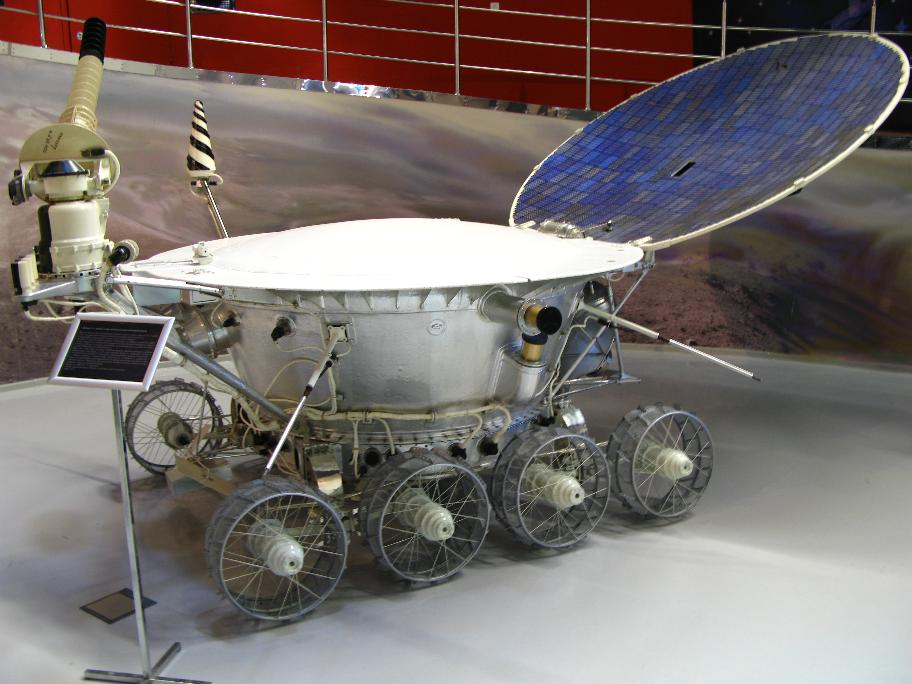
\includegraphics[width=0.45\textwidth]{Figures/RoverLunokhod1.jpg}
        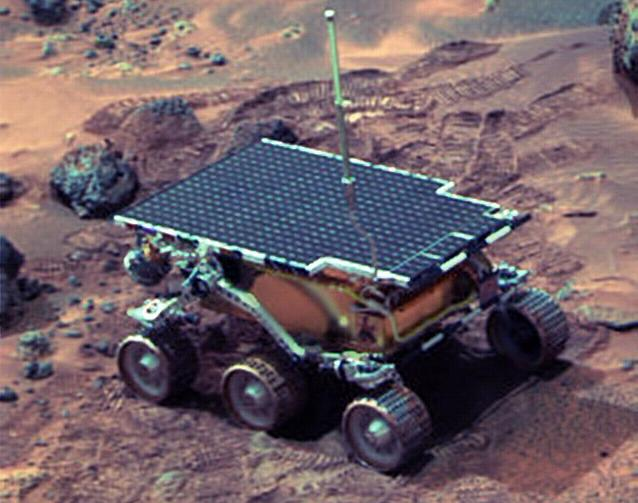
\includegraphics[width=0.45\textwidth]{Figures/RoverSojourner.jpg}
        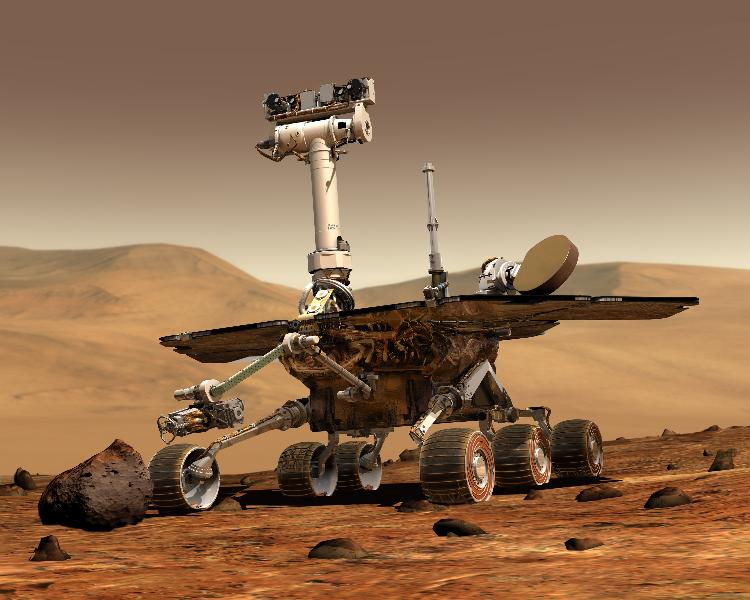
\includegraphics[width=0.45\textwidth]{Figures/RoverOpportunity.jpg}
        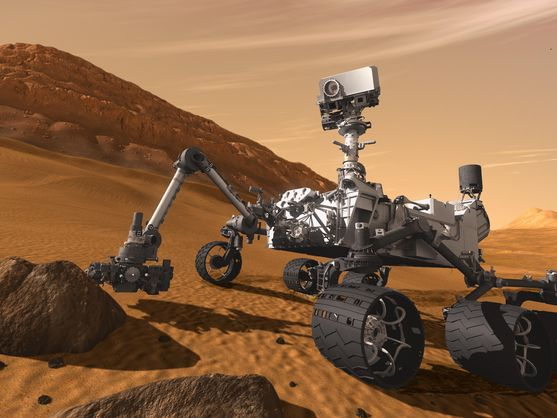
\includegraphics[width=0.45\textwidth]{Figures/RoverCuriosity.jpg}
      \end{figure}
    \end{column}
  \end{columns}
\end{frame}

\begin{frame}\frametitle{Los robots en el espacio (Humanoides)}
  Además de rovers, también hay desarrollo en robots de servicio para aplicaciones aeroespaciales\cite{bogue2012robots}:
  \begin{columns}
    \begin{column}{0.5\textwidth}
      \begin{figure}
        \centering
        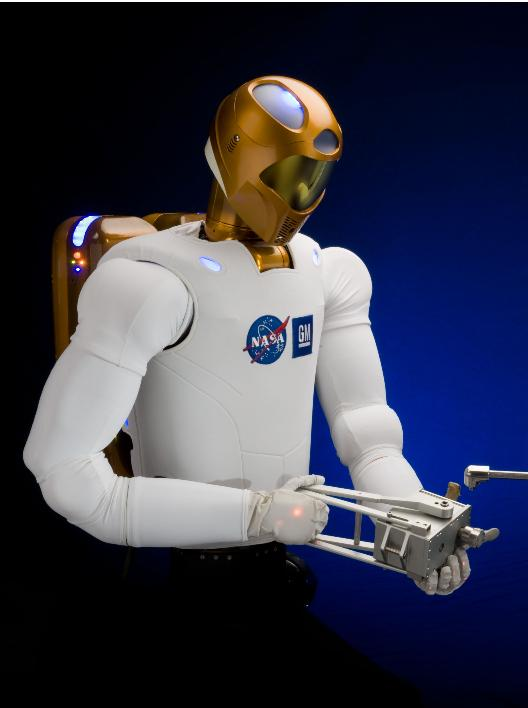
\includegraphics[width=0.45\textwidth]{Figures/RobotRobonaut.jpg}
        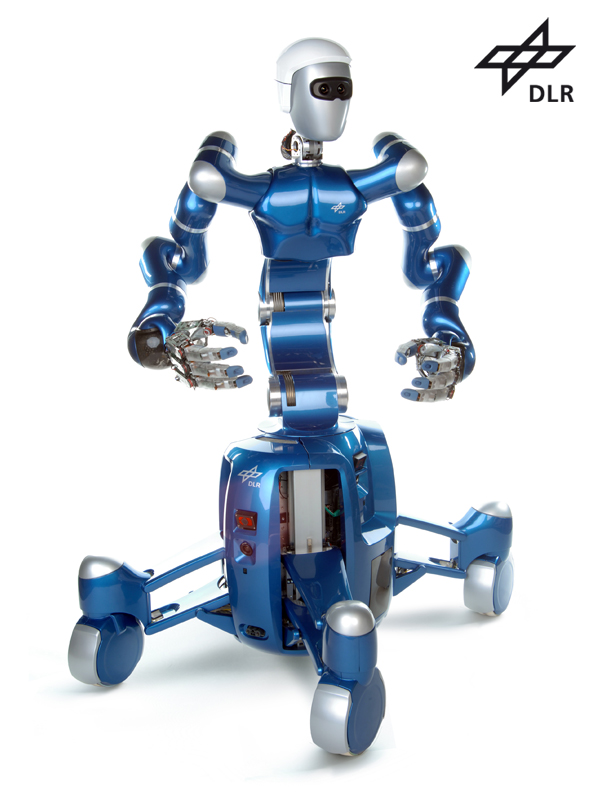
\includegraphics[width=0.45\textwidth]{Figures/RobotJustin.jpg}
      \end{figure}
    \end{column}
    \begin{column}{0.5\textwidth}
      \begin{itemize}
      \item Robonaut R2, desarrollado por DARPA/NASA, en la ISS en 2011$^1$
      \item Rollin'Justin, desarrollado por el DLR$^2$
      \end{itemize}
    \end{column}
  \end{columns}
  $^1$\footnotesize{\url{https://www.nasa.gov/robonaut2}}\\
  $^2$\footnotesize{\url{https://www.dlr.de/rm/en/desktopdefault.aspx/tabid-11427/}}
\end{frame}

\begin{frame}\frametitle{ROS en proyectos aeroespaciales}
  \begin{columns}
    \begin{column}{0.5\textwidth}
      \begin{itemize}
      \item ROS Space: La plataforma ROS con estándar aeroespacial para software$^1$
      \item Robonaut 2 y 5 utilizan ROS y tienen sus versiones en Gazebo$^2$
      \item Astrobee, desarrollado por la NASA utiliza ROS$^3$
      \item El proyecto VIPER (NASA) utiliza Gazebo para simulaciones$^4$ 
      \end{itemize}
    \end{column}
    \begin{column}{0.5\textwidth}
      \begin{figure}
        \centering
        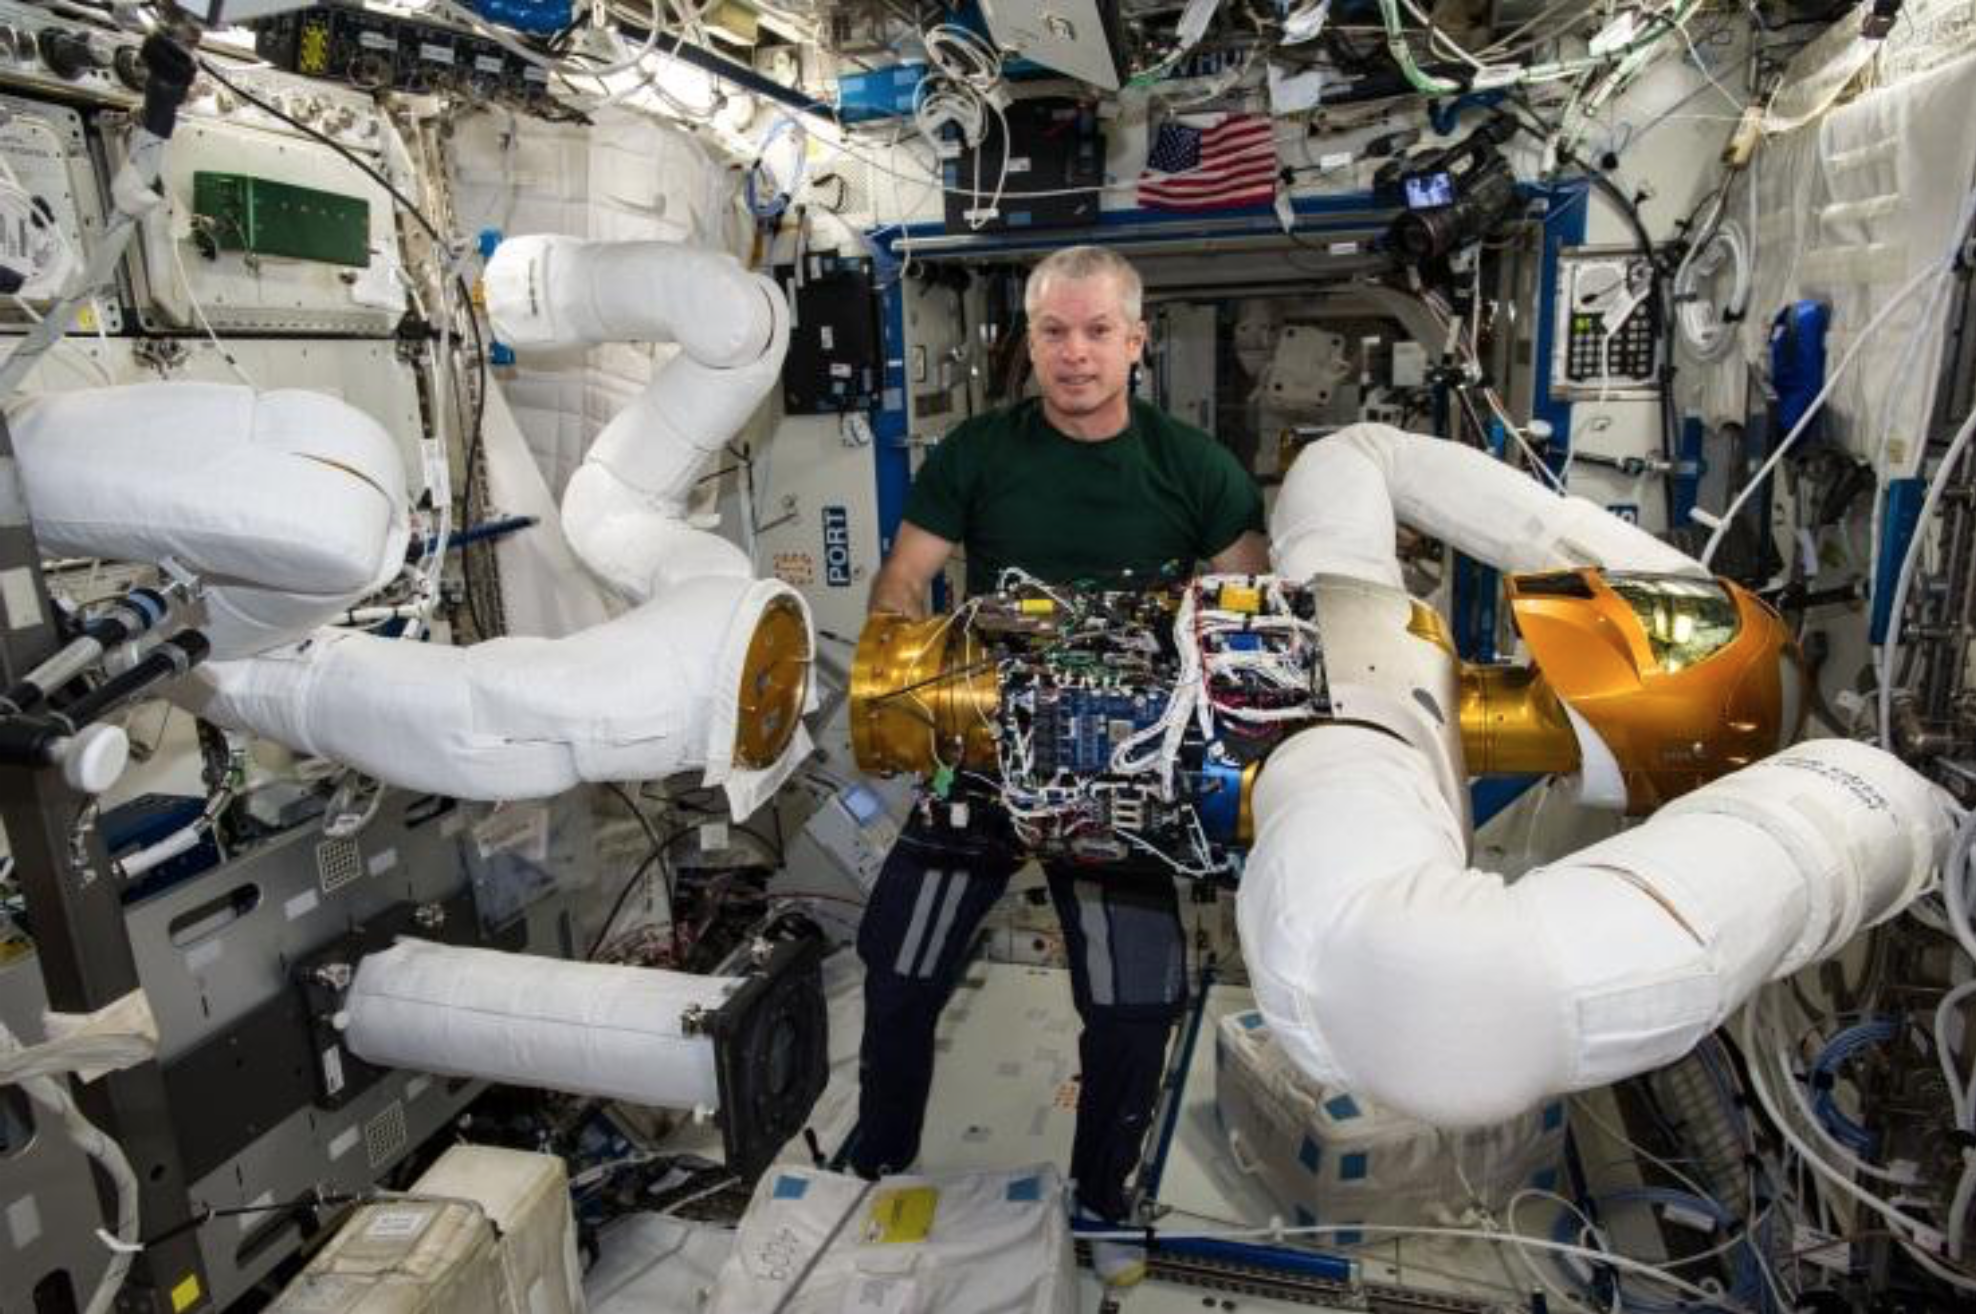
\includegraphics[width=0.45\textwidth]{Figures/ROSRobonaut.png}
        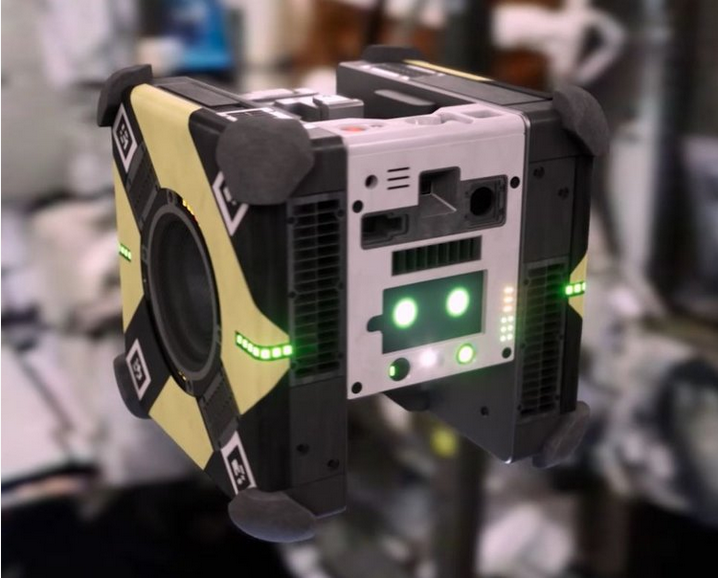
\includegraphics[width=0.45\textwidth]{Figures/ROSAstrobee.png}
        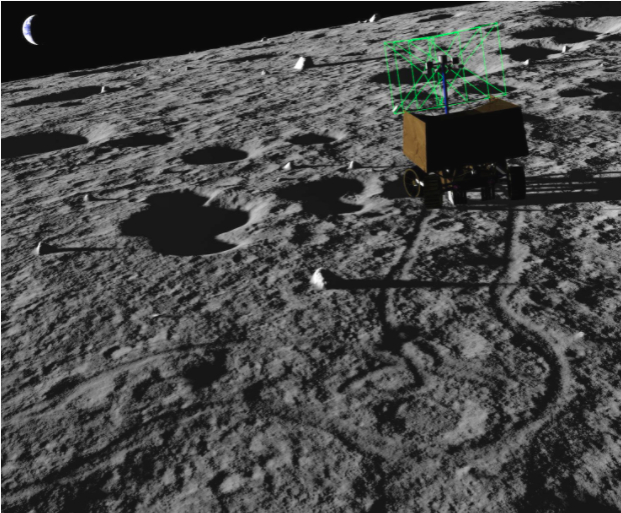
\includegraphics[width=0.45\textwidth]{Figures/ROSViper.png}
      \end{figure}
    \end{column}
  \end{columns}
  $^1$\footnotesize{\url{https://vimeo.com/649649866/37198994b5}}\\
  $^2$\footnotesize{\url{https://robots.ros.org/robonaut2/}}\\
  $^3$\footnotesize{\url{https://github.com/nasa/astrobee}}\\
  $^4$\footnotesize{\url{https://www.openrobotics.org/blog/2022/2/2/rosinspace}}
\end{frame}

\begin{frame}\frametitle{El robot Toyota HSR}
  El \textit{Human Support Robot} (HSR) de Toyota es una plataforma para investigación en robots de servicio.
  \begin{columns}
    \begin{column}{0.4\textwidth}
      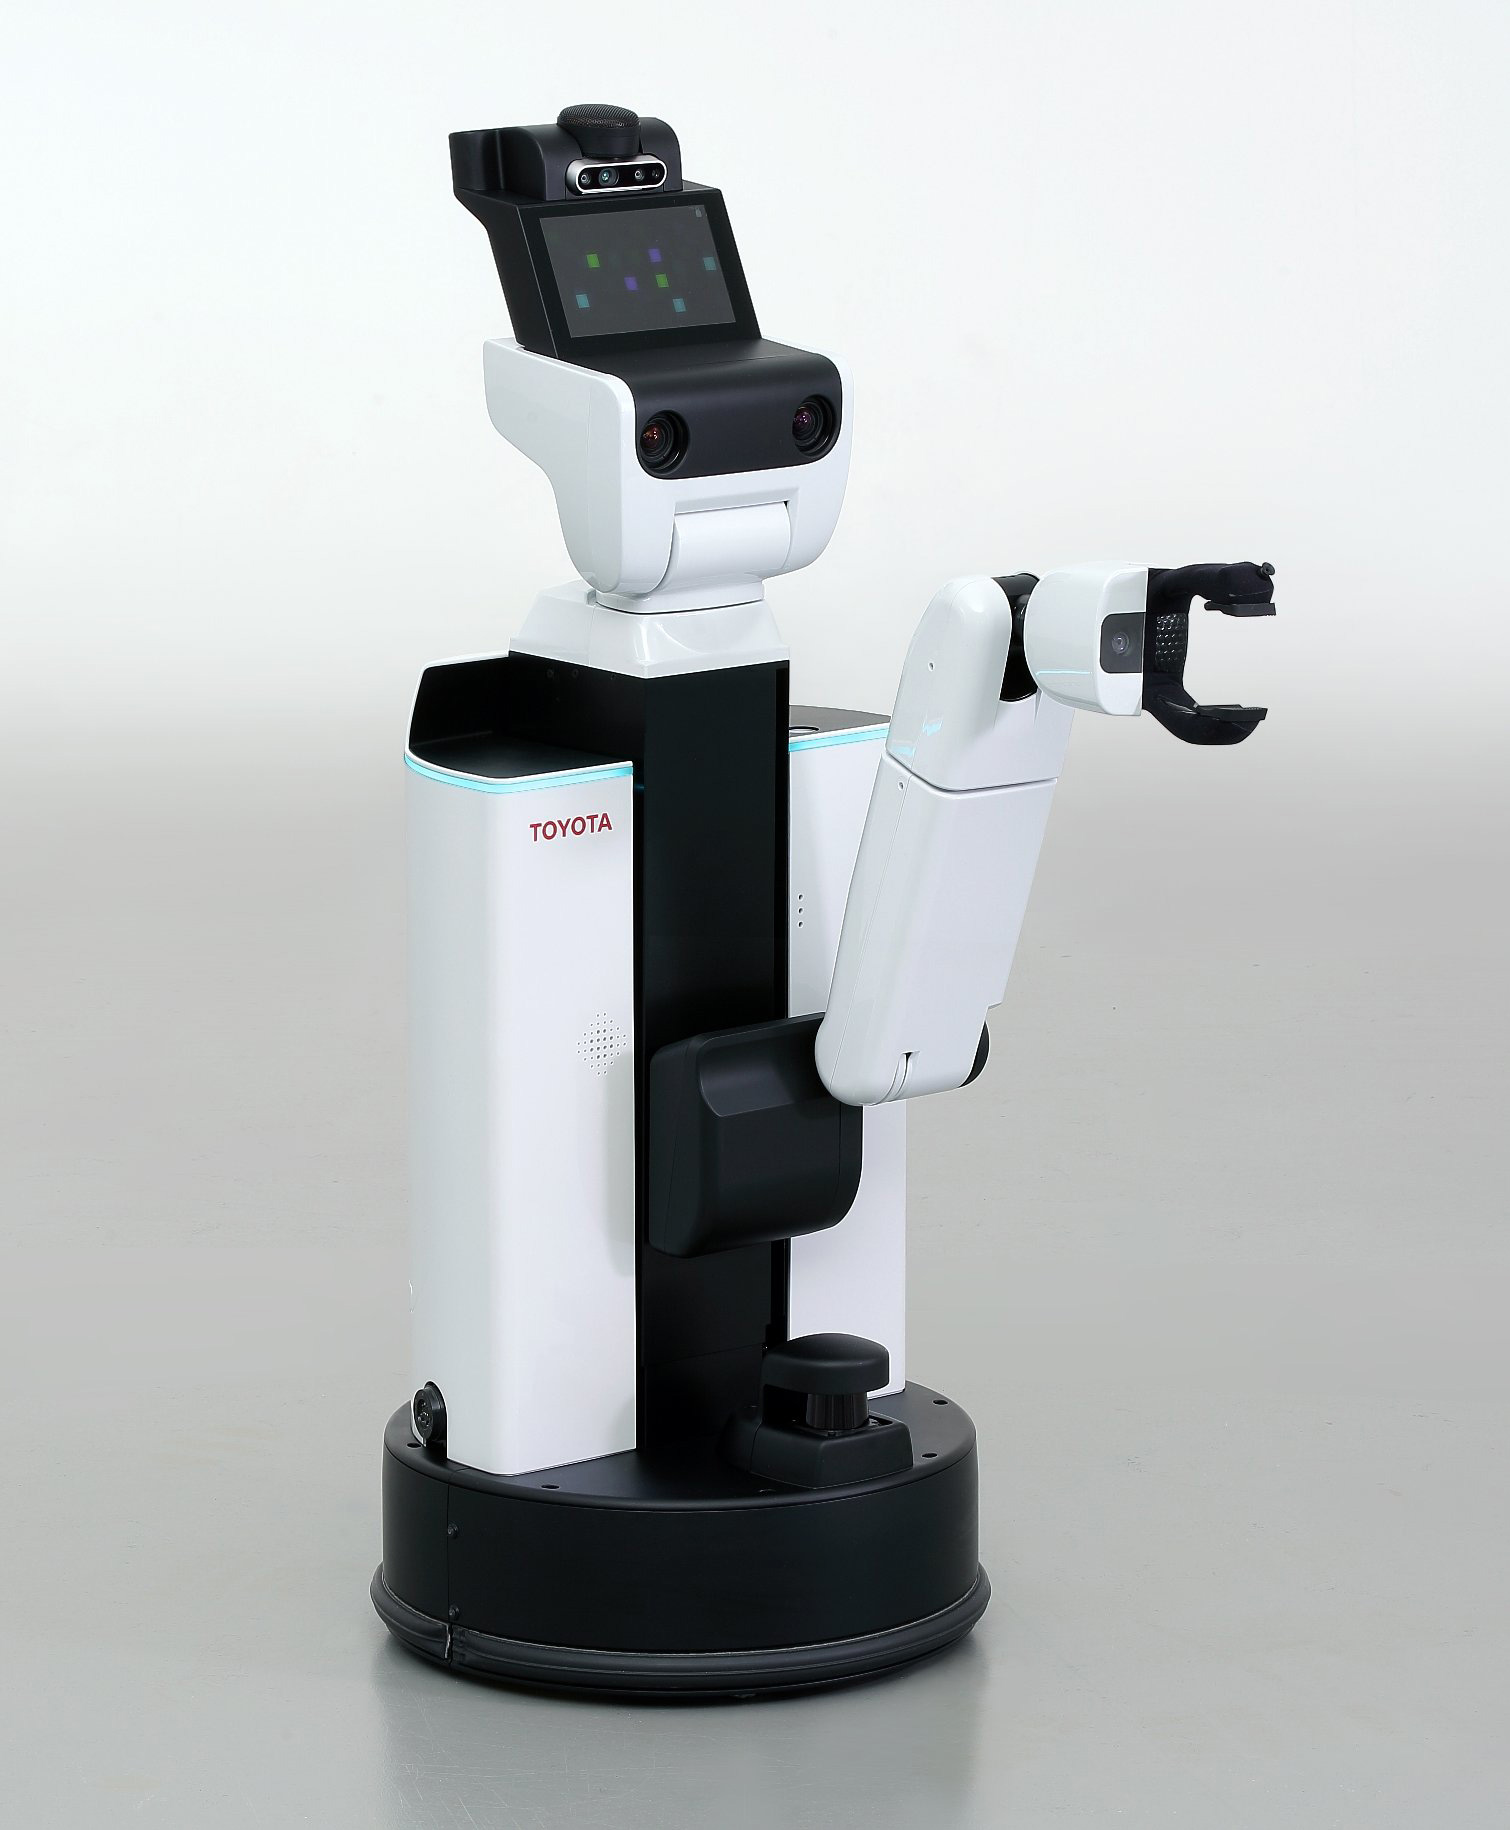
\includegraphics[width=0.9\textwidth]{Figures/HSR.jpg}
    \end{column}
    \begin{column}{0.6\textwidth}
      Hardware:
      \begin{itemize}
      \item Base móvil omnidireccional
      \item Manipulador de 5 DoF
      \item Cámaras RGB y RGB-D en la cabeza
      \item Cámara RGB en el efector final
      \item Lidar en la base móvil
      \item Bocinas y micrófono
      \end{itemize}
      Software: Arquitectura basada en ROS con las siguientes funcionalidades:
      \begin{itemize}
      \item Control de la base móvil
      \item Control del manipulador
      \item Acceso a los datos de los sensores mediante tópicos
      \end{itemize}
    \end{column}
  \end{columns}
\end{frame}

%%%%%%%%%%%%%%%%%%%%%
%%%%%%%%%%%%%%%%%%%%% Conceptos Básicos
%%%%%%%%%%%%%%%%%%%%%
\section{Conceptos Básicos}
\begin{frame}\frametitle{Contexto y definiciones}
  \begin{itemize}
  \item La palabra \textit{robot} tiene su origen en la obra \textit{Rossum's Universal Robots} del escritor checo $Karel \,\check{C}apeck$, publicada en 1921, y su significado es ``trabajo duro''.
  \item Latombe (1991) define un robot como un dispositivo mecánico versátil equipado con sensores y actuadores bajo el control de un sistema de cómputo \cite{Latombe1991MotionPlanning}.
  \item Arkin (1998) propone que un robot inteligente es una máquina capaz de extraer información de su ambiente y usar el conocimiento acerca de su mundo para moverse de manera segura y significativa, con un propósito específico \cite{Arkin1998BehBasedRobo}.
  \item Robótica es la ciencia que estudia la conexión inteligente entre la percepción y la acción. 
  \end{itemize}
\end{frame}

\begin{frame}\frametitle{Áreas de la Robótica}
  
  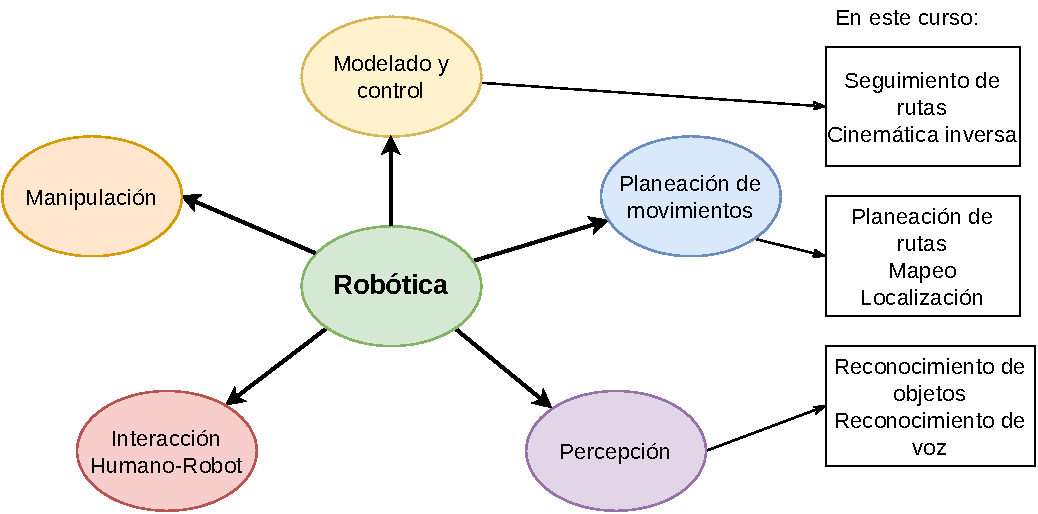
\includegraphics[width=0.9\textwidth]{Figures/RoboticsAreas.pdf}
\end{frame}

\begin{frame}\frametitle{Componentes de un robot}
  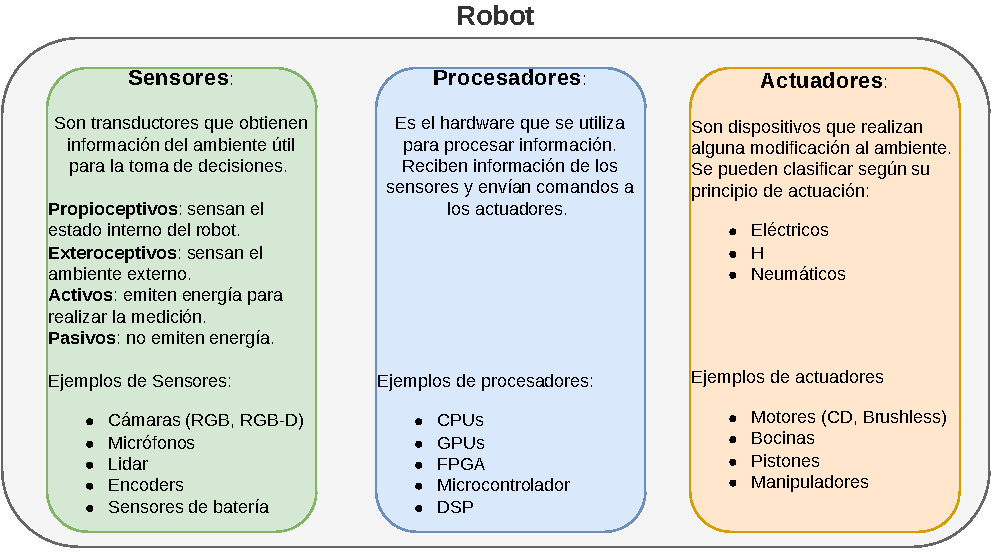
\includegraphics[width=0.9\textwidth]{Figures/RobotComponents.pdf}
\end{frame}

\begin{frame}\frametitle{Conceptos Básicos}
  \begin{itemize}
  \item \textbf{Configuración:} es la descripción de la posición en el espacio de todos los puntos del robot. Se denota con $q$.
  \item \textbf{Espacio de configuraciones:} es el conjunto $Q$ de todas las posibles configuraciones. 
  \item \textbf{Grados de libertad:} número mínimo de variables independientes para describir una configuración. En este curso, la base móvil del robot tiene 3 GdL, la cabeza tiene 2 GDL y cada brazo tiene 7 GDL más 1 GdL para el gripper. En total, el robot tiene 21 GdL. 
  \end{itemize}
  \textbf{Propiedades del robot:}
  \begin{itemize}
  \item \textbf{Holonómico:} el robot puede moverse instantáneamente en cualquier dirección del espacion de configuraciones. Comunmente se logra mediante ruedas de tipo \textit{Mecanum} u \textit{Omnidireccionales}. 
  \item \textbf{No holonómico:} existen restricciones de movimiento en velocidad pero no en posición. Son restricciones que solo se pueden expresar en términos de la velocidad pero no pueden integrarse para obtener una restricción en términos de posición. Ejemplo: un coche sólo puede moverse en la dirección que apuntan las llantas delanteras, sin embargo, a través de maniobras puede alcanzar cualquier posición y orientación. El robot de este curso es no holonómico. 
  \end{itemize}
\end{frame}

\begin{frame}\frametitle{Conceptos Básicos}
  \textbf{Propiedades de los algoritmos:}
  \begin{itemize}
  \item \textbf{Complejidad:} cuánta memoria y cuánto tiempo se requiere para ejecutar un algoritmo, en función del número de datos de entrada (número de grados libertad, número de lecturas de un sensor, entre otros).
  \item \textbf{Optimalidad:} un algoritmo es óptimo cuándo encuentra una solución que minimiza una función de costo.
  \item \textbf{Completitud:} un algoritmo es completo cuando garantiza encontrar la solución siempre que ésta exista. Si la solución no exite, indica falla en tiempo finito.
    \begin{itemize}
    \item Completitud de resolución: la solución existe cuando se tiene una discretización. 
    \item Completitud probabilística: la probabilidad de encontrar la solución tiende a 1.0 cuando el tiempo tiende a infinito.
    \end{itemize}
  \end{itemize}
  Una explicación más detallada se puede encontrar en el Cap. 3 de \cite{choset2005principles}.
\end{frame}

\begin{frame}\frametitle{Primitivas de la robótica}
Las tareas que puede llevar a cabo un robot se pueden clasificar en tres grandes conjuntos conocidos como primitivas de la robótica: sensar, planear y actuar.
  \begin{itemize}
  \item \textbf{Sensar: } extracción de información del ambiente interno o externo del robot.
  \item \textbf{Planear: } generación de subtareas y toma decisiones a partir de la información de los sensores y/o de alguna Representación intenra del ambiente.
  \item \textbf{Actuar: } modificación del ambiente con alguno de los dispositivos del robot. 
  \end{itemize}
\end{frame}

\begin{frame}\frametitle{Paradigmas de la robótica}
  \textbf{Paradigma jerárquico.} Las tres primitivas se realizan en forma secuencial.
  \begin{figure}
    \centering
    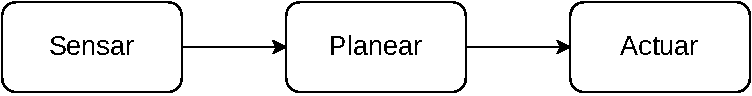
\includegraphics[width=0.7\textwidth]{Figures/ParadigmHierarchical.pdf}
  \end{figure}
  \begin{itemize}
  \item Fuerte dependencia de una representación interna del ambiente
  \item Tiempo de respuesta lento comparado con el paradigma reactivo
  \item Alto costo computacional
  \item Se pueden resolver tareas con alto nivel cognitivo
  \item Alta capacidad de predicción
  \end{itemize}
\end{frame}

\begin{frame}\frametitle{Paradigmas de la robótica}
  \textbf{Paradigma reactivo.} El sensado y la actuación se conectan directamente sin que haya de por medio una planeación.
  \begin{figure}
    \centering
    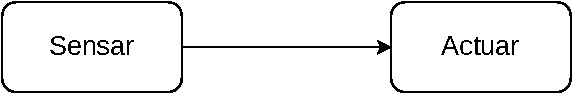
\includegraphics[width=0.5\textwidth]{Figures/ParadigmReactive.pdf}
  \end{figure}
  \begin{itemize}
  \item No requiere una representación interna del ambiente
  \item Tiempo de respuesta rápido comparado con el paradigma jerárquico
  \item Bajo costo computacional
  \item En general, no se pueden resolver tareas con alto nivel cognitivo
  \item Baja capacidad de predicción
  \end{itemize}
\end{frame}

\begin{frame}\frametitle{Paradigmas de la robótica}
  \textbf{Paradigma híbrido.} Tiene como objetivo utilizar las ventajas de ambos paradigmas, es decir, emplear comportamientos reactivos para que el robot responda rápidamente ante cambios en el ambiente sin perder la alta capacidad cognitiva y de predicción que brinda el paradigma jerárquico
  \begin{figure}
    \centering
    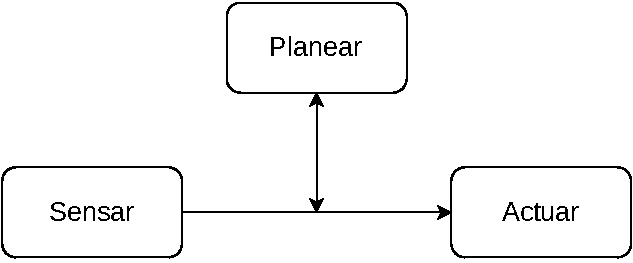
\includegraphics[width=0.5\textwidth]{Figures/ParadigmHybrid.pdf}
  \end{figure}
\end{frame}


%%%%%%%%%%%%%%%%%%%%%
%%%%%%%%%%%%%%%%%%%%% ROS
%%%%%%%%%%%%%%%%%%%%%
\section{ROS}
\begin{frame}\frametitle{La plataforma ROS}
  
\includegraphics[width=0.3\textwidth]{Figures/Ros_logo.png}
  \[\]
  \textbf{ROS (Robot Operating System) } es un \textit{middleware} de código abierto para el desarrollo de robots móviles.
  \begin{itemize}
  \item Implementa funcionalidades comúnmente usadas en el desarrollo de robots como el paso de mensajes entre procesos y la administración de paquetes.
  \item Muchos drivers y algoritmos ya están implementados.
  \item Es una plataforma distribuida de procesos (llamados \textit{nodos}).
  \item Facilita el reuso de código.
  \item Independiente del lenguaje (Python y C++ son los más usados).
  \item Facilita el escalamiento para proyectos de gran escala. 
  \end{itemize}
\end{frame}

\begin{frame}\frametitle{Conceptos}
  ROS se puede entender en dos grandes niveles conceptuales:
  \begin{itemize}
  \item \textbf{Sistema de archivos:} Recursos de ROS en disco
  \item \textbf{Grafo de procesos:} Una red \textit{peer-to-peer} de procesos (llamados nodos) en tiempo de ejecución.
  \end{itemize}
\end{frame}

\begin{frame}\frametitle{Sistema de archivos}
  \begin{columns}
    \begin{column}{0.5\textwidth}
      Recursos en disco:
      \begin{itemize}
      \item \textbf{Workspace:} carpeta que contiene los paquete desarrollados
      \item \textbf{Paquetes:} Principal unidad de organización del software en ROS (concepto heredado de Linux)
      \item \textbf{Manifiesto:} (\texttt{package.xml}) provee metadatos sobre el paquete (dependencias, banderas de compilación, información del desarrollador)
      \item \textbf{Mensajes (msg):} Archivos que definen la estructura de un \textit{mensaje} en ROS.
        \item \textbf{Servicios (srv):} Archivos que definen las estructuras de la petición (\textit{request}) y respuesta (\textit{response}) de un servicio. 
      \end{itemize}
    \end{column}
    \begin{column}{0.4\textwidth}
      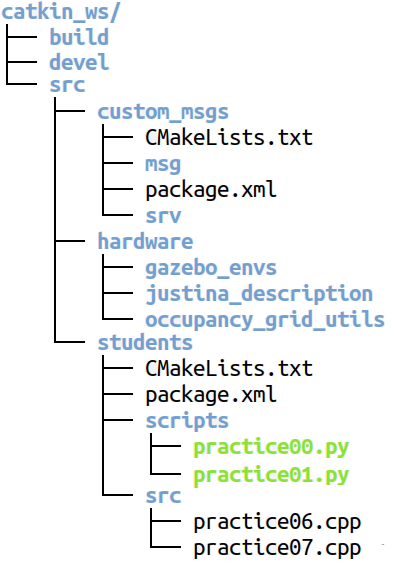
\includegraphics[width=\textwidth]{Figures/catkin_tree.png}
    \end{column}
  \end{columns}
\end{frame}

\begin{frame}\frametitle{Grafo de procesos}
  El grafo de procesos es una red \textit{peer-to-peer} de programas (nodos) que intercambian información entre sí. Los principales componentes del este grafo son:
  \[\]
  \begin{columns}
    \begin{column}{0.5\textwidth}
      \begin{itemize}
      \item master
      \item servidor de parámetros
      \item nodos
      \item mensajes
      \item servicios 
      \end{itemize}
    \end{column}
    \begin{column}{0.5\textwidth}
      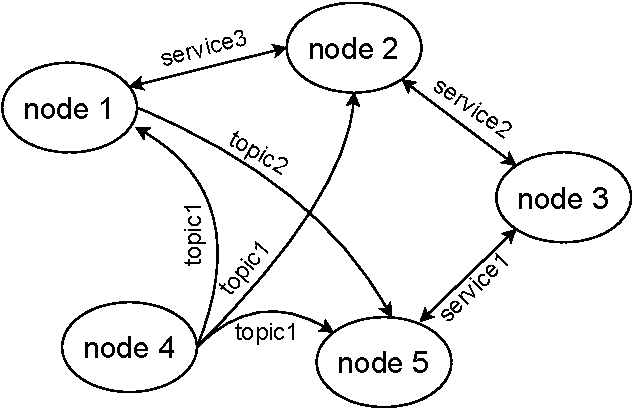
\includegraphics[width=\textwidth]{Figures/RosGraph.pdf}
    \end{column}
  \end{columns}
\end{frame}

\begin{frame}\frametitle{Tópicos y servicios}
  Los nodos (procesos) en ROS intercambian información a través de dos grandes patrones:
  \begin{columns}
    \begin{column}{0.6\textwidth}
        \begin{itemize}
        \item \textbf{Tópicos}
          \begin{itemize}
          \item Son un patrón $1:n$ de tipo \textit{publicador/suscriptor}
          \item Son no bloqueantes
          \item Utilizan estructuras de datos definidas en archivos \texttt{*.msg} para el envío de información
          \end{itemize}
        \item \textbf{Servicios}
          \begin{itemize}
          \item Son un patrón $1:1$ de tipo \textit{petición/respuesta}
          \item Son bloqueantes
          \item Utilizan estructuras de datos definidas en archivos \texttt{*.srv} para el intercambio de información. 
          \end{itemize}
        \end{itemize}
    \end{column}
    \begin{column}{0.4\textwidth}
      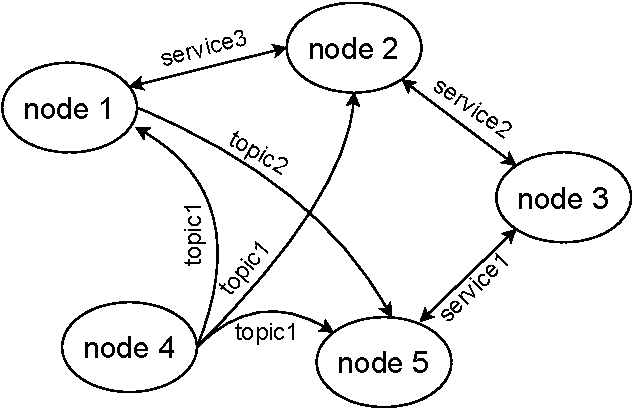
\includegraphics[width=\textwidth]{Figures/RosGraph.pdf}
    \end{column}
  \end{columns}
  \[\]
  Para mayor información:
  \begin{itemize}
  \item Tutoriales \url{http://wiki.ros.org/ROS/Tutorials}
  \item Koubâa, A. (Ed.). (2020). Robot Operating System (ROS): The Complete Reference. Springer Nature
  \end{itemize}
\end{frame}

%%%%%%%%%%%%%%%%%%%%%
%%%%%%%%%%%%%%%%%%%%% Ejercicio
%%%%%%%%%%%%%%%%%%%%%
\section{Ejercicios}
\begin{frame}[containsverbatim]\frametitle{Ejercicio 1}
  \begin{enumerate}
  \item Investigar para qué sirve el mensaje \texttt{LaserScan}
  \item Investigar para qué sirve el mensaje \texttt{Twist}
  \item Buscar para qué sirven los comandos: \texttt{rosrun}, \texttt{rostopic list} y \texttt{rostopic echo}
  \item Abra el archivo \texttt{catkin\_ws/src/exercises/scripts/exercise01.py} y agregue el siguiente código en la línea 27:
  \begin{lstlisting}[language=Python,firstnumber=27]
n = int((msg.angle_max - msg.angle_min)/msg.angle_increment/2)
obstacle_detected = msg.ranges[n] < 1.0
  \end{lstlisting}
  En el mismo archivo, en la línea 49, agregue el siguiente código:
  \begin{lstlisting}[language=Python,firstnumber=49]
msg_cmd_vel = Twist()
msg_cmd_vel.linear.x = 0 if obstacle_detected else 0.3
pub_cmd_vel.publish(msg_cmd_vel)
\end{lstlisting}
\item Corra el programa con los comandos:
  \begin{verbatim}
$ source ~/CIRE2022/catkin_ws/devel/setup.bash
$ rosrun exercises exercise01.py
\end{verbatim}
  \item Describir qué hace el programa y, de ser posible, realice un diagrama de flujo o esquema similar. 
  \end{enumerate}
\end{frame}

\bibliographystyle{abbrv}
\bibliography{References}
\begin{frame}
  \Huge{Gracias}
  \[\]
  \Large{Contacto}
  \[\]
  \large
  Dr. Marco Negrete\\
  Profesor Asociado C\\
  Departamento de Procesamiento de Señales\\
  Facultad de Ingeniería, UNAM.
\[\]
mnegretev.info\\
marco.negrete@ingenieria.unam.edu\\
\end{frame}
\end{document}
